% Inbuilt themes in beamer
\documentclass{beamer}
\usepackage{tikz}
\usepackage{pgfpages}

% Theme choice:
\usetheme{kellentheme}

% Title page details: 
\title{Temporal Difference Flows \cite{farebrotherTemporalDifferenceFlows2025}} 
\author{Kellen Kanarios}
\date{\today}
\logo{
    % 
\includegraphics[width=0.05\linewidth]{figures/umich-m.png}
}


\setbeamertemplate{footline}[myfootline]
\begin{document}

% Title page frame
\begin{frame}
    \titlepage 
\end{frame}

\part{Background}

\begin{frame}{Outline}
    \tableofcontents
\end{frame}

\section{Diffusion Recap}
\subsection{Continuity Equation}
\begin{frame}{Continuity Equation}
    \begin{minipage}{0.5\textwidth}
        \begin{block}{Def.}
            \vspace*{-.5cm}
            \[ \mathrm{d}X_t = v(t, X_t)\mathrm{d}t \]
        \end{block}
    \end{minipage}
    \begin{block}{Eqn.}
        \vspace*{-.5cm}
        \begin{equation}\label{eqn:continuity}
            \frac{\partial}{\partial t}\boldsymbol{p} + \nabla_x (\boldsymbol{p} \cdot \boldsymbol{v}) = 0
        \end{equation}
    \end{block}
    \begin{exampleblock}{Proof sketch.}
        \vspace*{-0.8cm}
        \begin{align}
            \frac{\partial}{\partial t}(p_t(X_t)) &= \frac{\partial}{\partial t} p_t(X_t) \mathrm{d}X_t \\
            x &= y \\
            x &= y \\
            x &= y
        .\end{align}
    \end{exampleblock}
\end{frame}
\section{Flow Matching}
\subsection{Flow vs. Score}
% Lists frame
\begin{frame}{Diffusion vs. Flow Matching}
\begin{columns}

  \begin{column}{0.48\textwidth}
      \begin{alertblock}{Diffusion Models}
      \begin{itemize}
        \item Learn the score \( \nabla \ln p_t \)
        \item Corresponds to one particular choice of vector field
      \end{itemize}
    \end{alertblock}
  \end{column}

  \begin{column}{0.48\textwidth}
      \begin{exampleblock}{Flow Models}
      \begin{itemize}
        \item Directly learn the vector field \( v_t \)
        \item Corresponds to one choice of ``flow''
      \end{itemize}
    \end{exampleblock}
  \end{column}
\end{columns}
\begin{tikzpicture}[remember picture, overlay]
  \draw[->, thick, dashed, red]
  (2.5, 1.5) to[bend left=30] (8, 1.5);
\end{tikzpicture}
\note{testing if this note works}
\end{frame}

\begin{frame}{Why Flows?}
    \begin{block}{Anecdotally}
        \begin{itemize}
            \item{\footnotesize \emph{The OT path’s conditional
                vector field has constant direction in time and is arguably simpler to fit with a parametric model. \cite{lipmanFlowMatchingGenerative2023}}}
            \item{\footnotesize \emph{The deterministic
                nature of ODEs equips flow-matching methods with simpler learning objectives and faster inference speed \cite{zhengIntentionConditionedFlowOccupancy2025}}}
        \end{itemize}
    \end{block}
    \vspace*{.5cm}
\begin{figure}
    \hspace*{-.5cm}
    \begin{minipage}{0.50\linewidth}
    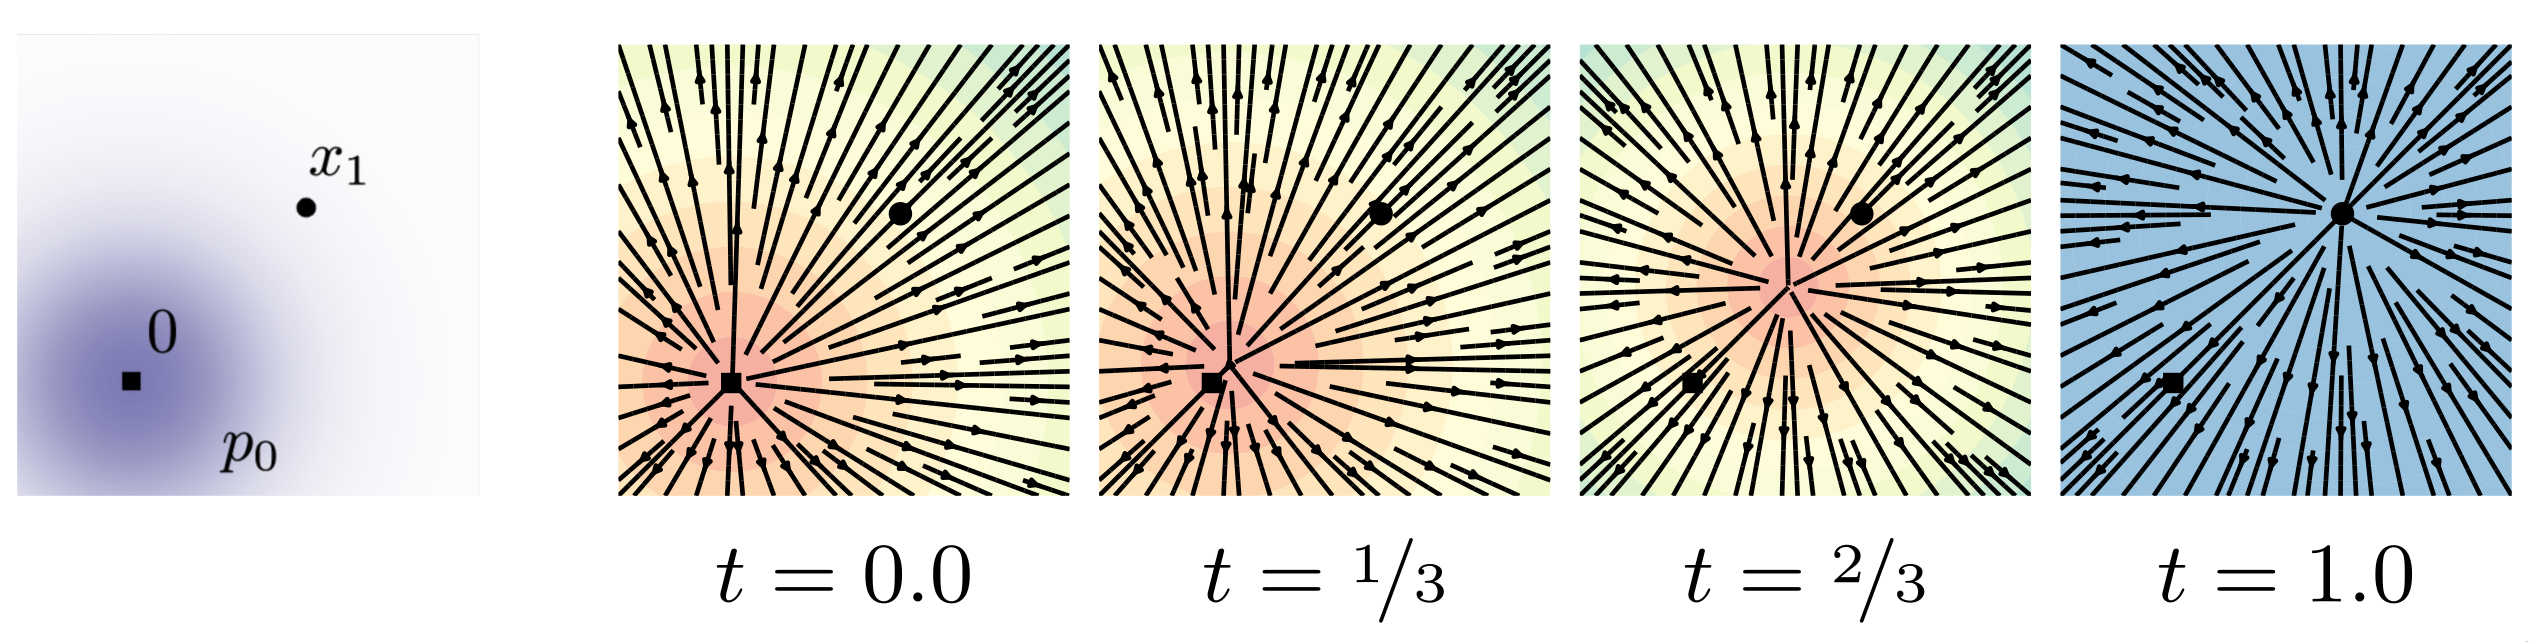
\includegraphics[width=1.2\linewidth]{figures/conditional-score.png}
    \hspace*{2.5cm}
    {\footnotesize Conditional score}
    \end{minipage}
    \hspace*{1cm}
    \begin{minipage}{0.39\linewidth}
    \centering
    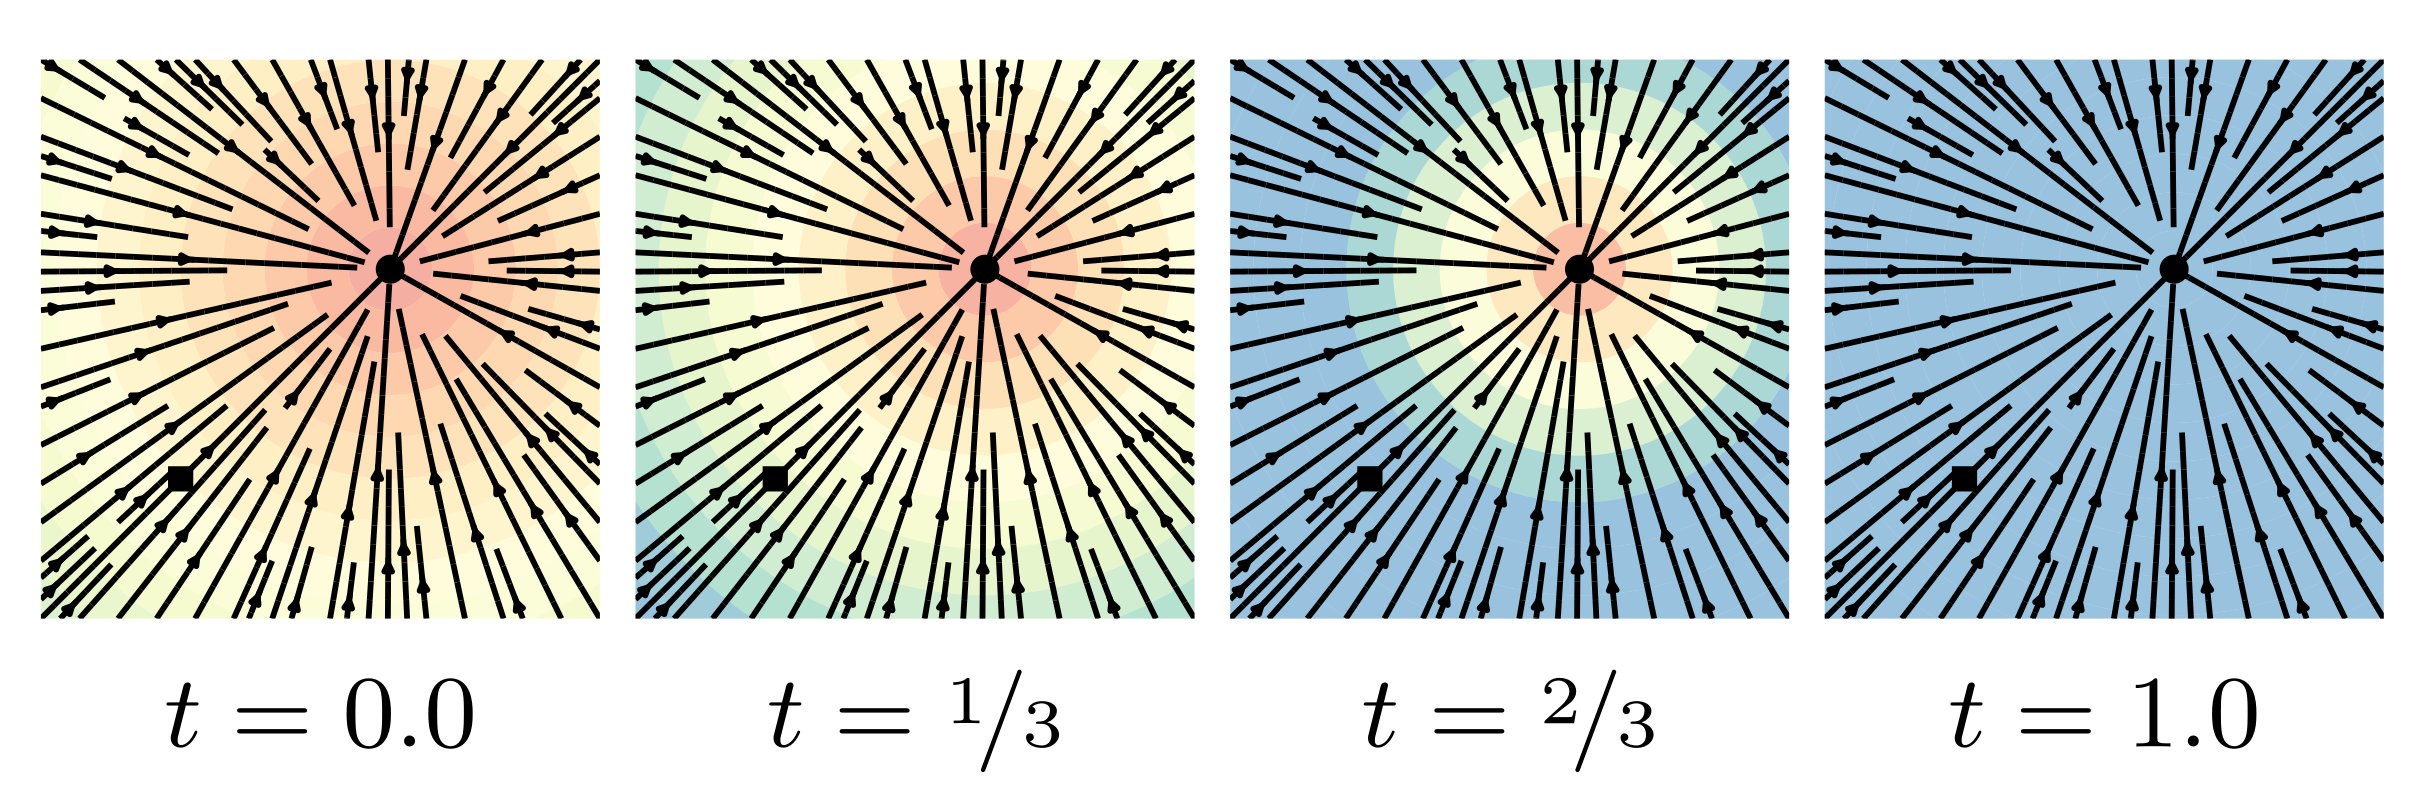
\includegraphics[width=1.2\linewidth]{figures/conditional-vector-field.png}
    {\footnotesize Conditional vector field}
    \end{minipage}
\end{figure}
\end{frame}

\subsection{Learning the Flow}
\begin{frame}{Naive Loss + Problems}
    \begin{minipage}{0.46\textwidth}
        \begin{block}{Defs.}
            \begin{itemize}
                \item \( p_t \)
                \item \( u(t, \cdot) \)
            \end{itemize}
        \end{block}
    \end{minipage}
    \begin{block}{Flow Model Loss}
        \[ \mathcal{L}_{\text{\tiny FM}}(\theta) = \mathbb{E}_{t, p_t(x)} \|v_{\theta}(t, x) - u(t, x)\|^2 \]
    \end{block}
    \onslide<2->{
    \begin{alertblock}{Question}
        \centering
        How to sample from \( p_t \), or compute \( u(t, \cdot) \)?
    \end{alertblock}
    }
    \onslide<3->{
    \begin{exampleblock}{Answer}
        \centering
        We don't have to!!!!
    \end{exampleblock}
    }
\end{frame}

\begin{frame}{Conditioning Trick}
    \begin{minipage}{0.46\textwidth}
        \begin{block}{More defs.}
            \begin{itemize}
                \item \( \frac{\mathrm{d}}{\mathrm{d}t}\psi_t(x) = u(t, \psi_t(x)) \)
            \end{itemize}
        \end{block}
    \end{minipage}
\end{frame}

\begin{frame}{Equivalence of loss functions}
    
\end{frame}
\begin{frame}{Example: Optimal Transport}
    For \( \psi_t(x) = \mu_t(x_{1}) + x \sigma_t(x_{1}) \), we consider
    \begin{align*}
        \mu_t = tx_{1}, \quad \sigma_t(x) = 1 - (1 - t)\sigma_{\min}
    .\end{align*}
    Recall
    \begin{align*}
        \frac{\mathrm{d}}{\mathrm{d}t} \psi_t(x) = u(\psi_t(x) \mid X_{1})
    .\end{align*}
\end{frame}

\section{Application to Reinforcement Learning}
\begin{frame}{Long Horizon Problems Are Hard}
    \begin{block}{\cite{parkQlearningNotScalable2025}}
        \centering
        \vspace*{-1cm}
        \emph{\textbf{Seohong Park}; Q learning is not yet scalable}
    \end{block}
    \begin{figure}
        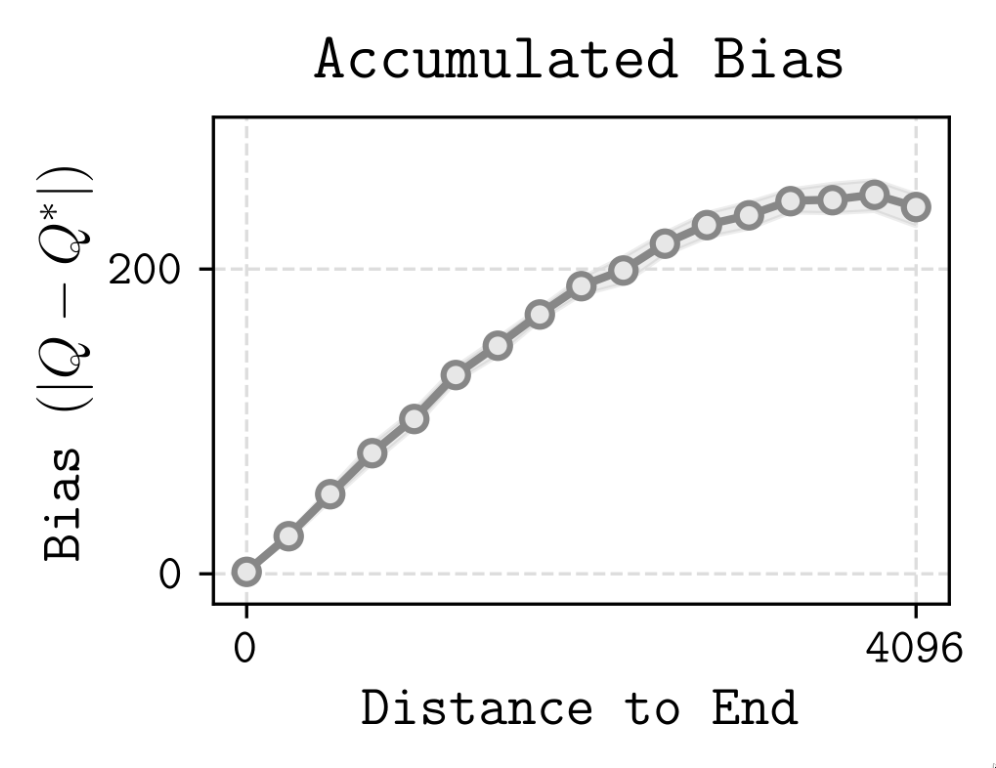
\includegraphics[width=0.5\linewidth]{figures/bias_accumulation.png}
    \end{figure}
    \begin{align*}
\mathbb{E}_{(s,a,r,s')\sim \mathcal{D}}\bigg[\Big(Q_\theta(s,a)-\underbrace{\big(r+\gamma \max_{a'}Q_{\bar{\theta}}(s',a')\big)}_{\texttt{Biased}}\Big)^2\bigg]
    .\end{align*}
\end{frame}
\subsection{Successor Measures}
\begin{frame}{Successor Measure}
    
\end{frame}


\begin{frame}{References}
    \bibliographystyle{alpha}
    \bibliography{references}
\end{frame}

\end{document}
